\chapter{外文资料的调研阅读报告或书面翻译}
\label{cha:CN}
\title{Zooids: 用于集群交互的积木}

\begin{figure}[htbp]
    \centering
    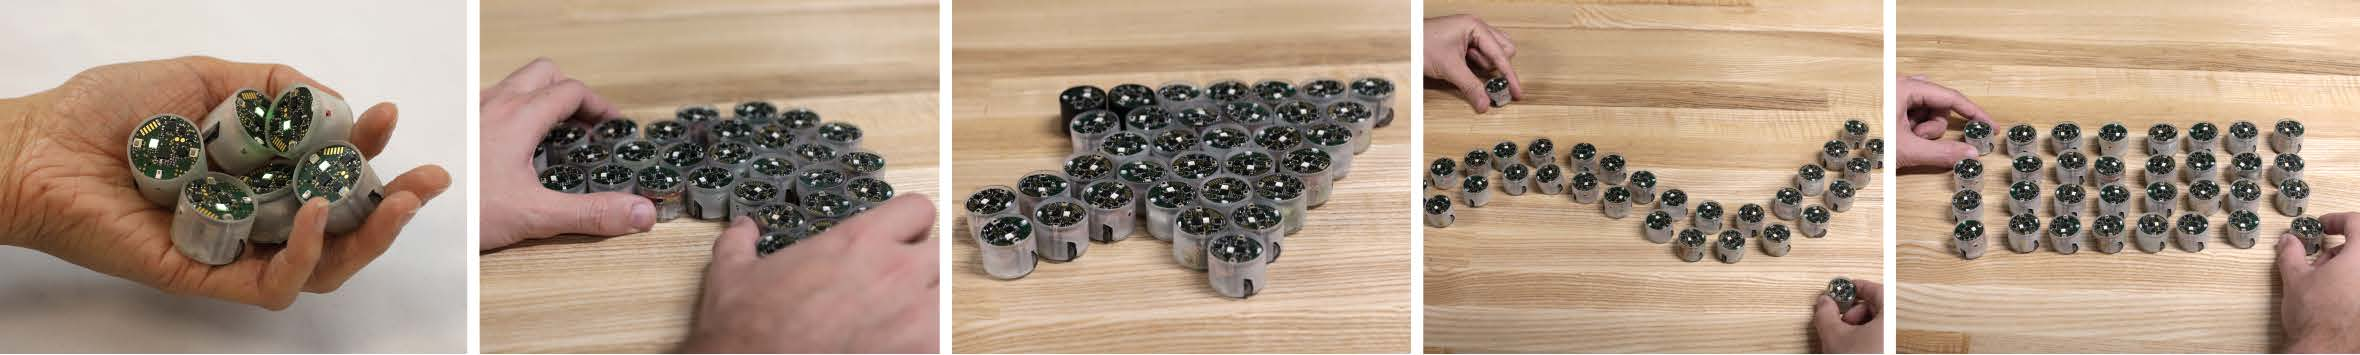
\includegraphics[width=\columnwidth]{zooids-1.jpg}
    \caption*{图~1\hskip1em Zooids可以被持有,可以集体或单独被操纵,表现为物理像素,充当控制器,并且可以在控制下动态移动。 它们是被称为群体交互界面的新型用户界面的积木单元。}
    \label{fig:headfigure}
\end{figure}

{\heiti 摘要:} 本文介绍了集群交互,这是一类新型的人机界面,由许多能够显示和交互的自主机器人组成。我们设计的Zooids是用于开发桌面集群交互的开源软硬件平台。该平台包括一组直径为2.6 cm的定制设计轮式微型机器人,一个无线电基站,一个用于光学跟踪的高速DLP结构光投影仪以及一个用于应用程序开发和控制的软件框架。我们通过使用Zooids开发的一组应用场景说明了桌面集群交互用户界面的潜力,并讨论了集群交互用户界面特有的设计注意事项。

{\heiti 关键词:} 集群用户界面; 实物用户界面。

\section{简介}

本文有助于使伊凡·萨瑟兰(Ivan Sutherland)“一个计算机可以控制物质存在的房间”的终极显示愿景成为现实,以及石井浩史(Hiroshi Ishii)的“人们可以与之交互的能够动态改变形式的新型原子”的愿景[26]。

近来,萨瑟兰(Sutherland)和石井(Ishii)的愿景已迈出了重要的一步,尤其是通过对驱动有形物体[48、50、78]和形状显示[55、56、15]的研究。但是,当前的系统受到许多限制。首先,被致动的桌面有形物品通常仅支持操纵和致动一些(例如3-4)固体物体,这不足以模拟可以改变形状的物理物质。另一方面,形状显示试图获得可以变形和驱动的表面,但是当前的实现并不支持任意的物理拓扑。此外,传统上,两种类型的系统都主要将物理对象用作输入,而输出几乎总是通过单独的基于像素的显示技术来提供。尽管视频投影覆盖图允许输入和输出在空间上重合[12],但它们仅提供有限的物理感[5]。同样,许多这样的系统需要笨重的硬件或显示器才能运行,因此主要是要在虚拟环境中运行,而不是嵌入我们自己的物理世界中[24,77]。

我们的研究工作是通过引入Zooid和大量用户界面来填补当前用户界面技术的空白(见图1)。 Zooid是一种硬件和软件系统:具有位置和触摸感应功能的小型轮式机器人,可以通过用户操作和计算机控制自由地布置和重新放置在任何水平面上。

Wikipedia中将“Zooid”定义为“属于动物群体的单个动物。Zooids是多细胞的。Zooids基于群机器人[10,68]的工作,增加了交互性和速度,它们的结构类似于其他孤独动物的结构。群体用户界面是使用自我推进的物理对象(例如微型机器人)的集合构建的界面,这些对象可以共同移动并对用户输入做出反应。群体用户界面可以看作是Sutherland和Ishii基于可编程物质的用户界面的未来派愿景的粗粒度版本。

由于Zooids具有在空间上自由,快速地重新配置自身的能力,因此,Zooids的集合可以充当显示器并提供有意义的用户输出。由于它们能够感知用户的动作,因此动物小动物还可以支持丰富的输入。例如,用户可以使用“扫动”手势一次移动Zooids,或者一次操纵许多Zooids[35]。可以在应用程序端实现复杂的交互行为,例如,动物类可以充当控件或操纵其他动物类的句柄;他们甚至可以移动其他轻型物体。同时,由于所有输入和输出都可以通过相同的物理元素进行调节,因此该系统能够实现输入和输出之间的完全融合,并提供物理操作的完整体验。最后,该系统相对轻巧,仅需使用紧凑的DLP投影仪(122毫米115毫米48毫米)进行光学跟踪。Zooids可以在任何水平表面上操作(例如,一张纸,凌乱的办公桌,餐桌或游戏板),从而可以将大量的用户界面与日常的物理环境融合在一起。为了刺激对群体用户界面的未来研究,我们以开源和开放硬件的形式分发了Zooids桌面群体用户界面平台。

总而言之,我们的贡献是:

\begin{itemize}
    \item 群体用户界面的有效定义,包含多个已实现的示例,
    \item 第一个用于实验桌面群用户界面的开源硬件/软件平台,
    \item 一组场景来说明我们的系统和桌面群体用户界面通常提供的前所未有的可能性,
    \item 关于群体用户界面的一些一般设计原理和设计挑战的讨论。
\end{itemize}

此外,Zooids有以下优点:

\begin{itemize}
    \item 与先前启动的有形用户界面可以共存,
    \item 既可以充当单个对象,又足够小以充当物理显示器的“像素”,
    \item 可以单独或集体操作,包括使用标尺等物理工具,
    \item 重量轻,可以在任何水平表面上操作,并且具有较低的成本:现在每个约50美元,如果批量生产,则为20美元。
\end{itemize}

\section{背景}

我们的工作涉及几个研究领域,即:桌面有形用户界面,形状显示,群机器人和数据物理化。

\subsection{桌面有形用户界面}

尽管有形用户界面(TUI)有许多不同的形式(包括传感器和执行器的模块化组件[19,40]),但桌面TUI尤其常见。

桌面TUI允许用户通过移动平面桌面上的物理对象(有形)与数字信息进行交互[72,73]。这些系统已用于一系列应用,例如系统工程控制[51],音乐作品[52],城市规划[74]和教育[23]。

传统桌面TUI的一个局限性是数字对象与物理对象之间的单向映射-如果前者发生变化,后者可能会变得不一致[26]。已经提出了许多技术来激活有形物体,包括2D门架[6,38],电磁体阵列[48,50,78、76],超声波换能器阵列[42],静电的吸引力[80,4],振动[57,81]和移动机器人[60,30、58、47、43、53、49]。这些系统还通过多种方式支持位置跟踪,例如使用LED或标记的摄像头(包括使用光学多点触摸台的摄像机)进行光学跟踪或基于投影仪的跟踪。有形物品的大小从硬币大小[48]到10厘米[53]不等。

人们已经在可动的桌面TUI上探索了多种交互技术,主要是基于每只手的单个有形物体的直接操纵[48],或者通过多点触摸输入[53]对小群可移动物体的直接操纵。 Patten [50]探索了将被动工具与可驱动有形物体结合使用来指定计算约束。其他研究人员在驱动的有形物体上增加了垂直位移等尺寸[43]。这些有效的有形物体在互动时可以通过在用户的手沿表面平移时直接对其施加力来提供触觉反馈[48、41]。由于远程对象可以保持同步[6,58],因此驱动的TUI还为远程协作提供了机会。

桌面TUI的设计空间很大,已经进行了很多探索。但是,先前的系统尚未考虑与许多(例如10、30或更多)小的驱动有形物体进行交互,我们展示了这种交互作用为新颖的交互作用和应用打开了可能性。同样,在许多以前的系统中[48、50、60、58、47、43、53、49、81],有形与图形显示结合使用,因此,有形主要用作数字信息的句柄。我们对用户界面感兴趣,在用户界面中,有形实体不仅用作控制器,还用作数字内容的表示。

\subsection{实体显示和可编程物质}

形状显示是涉及物理表面或体积的用户界面,可以感知用户输入,并且其几何形状可以由计算机控制[56,61]。许多此类系统支持使用电动棒[54、39、15]阵列对2.5D表面进行离散形状控制,而其他系统则支持使用气动或液压致动[14、82]或形状记忆合金进行连续形状控制[61]。当前,这些系统中的许多系统需要重型设备,并且仅允许对物理几何形状和拓扑进行有限的控制。特别是,以前的系统都无法模拟单独的,分离的物理对象。

这些研究工作部分地受到了Sutherland和Ishii之前讨论的愿景的启发,在这些愿景中,计算机将能够重新配置物理物质以重建任何物理形状。机器人技术和材料科学等其他领域也对实现“可编程物质”的梦想感兴趣,但到目前为止,大多数进展仅是理论上的[18,64]。工作原型依赖于群体机器人技术,我们将在后面讨论。

\subsection{集群机器人}

群体机器人是从自然群体中提取的,在自然群体中,鸟类或蚂蚁等社交动物可以根据简单的规则通过相互移动和交互来产生复杂的集体行为。迄今为止,已实施的最大的机器人群包括多达1,000台机器人,尽管它们移动缓慢(约1厘米/秒,而动物群的速度约为50厘米/秒)[63]。我们的论文是从过去对群体机器人技术的研究中得到启发的[10,9],但是尽管群体机器人技术领域一直最关注如何使用分布式智能和完全自治的代理来模仿群体行为,但我们专注于与机器人的直接物理交互。小群机器人,HCI应用程序,并采用集中式系统来协调机器人。

机器人技术的研究人员已开始开发与群体机器人进行交互的方法,但大多数方法仅在鼠标操作的计算机模拟中进行了测试[29,31]。阿隆索-莫拉(Alonso-Mora)及其同事研究了群体机器人作为物理显示器的用途[2],最近扩展了他们的系统,以通过素描[21],手持平板输入[20]和空中手势[3]支持交互。他们的系统与Zooids共享许多功能,但我们的论文重点是对群体机器人进行直接的有形操纵,并探讨了更广泛的应用场景。

最近,Rubens等人[62]描述了一种基于无人机的空中3D物理显示系统,用户可以通过直接操纵无人机进行交互。尽管他们的目标是最终收敛到群体用户界面,但是每架无人机都很大(8.9厘米),并且由于湍流问题,可同时使用的无人机数量受到限制-他们的原型机目前由3架无人机组成。无人驾驶飞机100 [16]项目涉及一百个称为“垃圾桶”的无人机。每个都有灯光,可以在三个维度上定位,从而形成了能够显示动态图像的编排群。但是,较大的操作量会阻止直接操作。

\subsection{数据实体化}

基于围绕体现和分布式认知的认知科学研究,最近对围绕物理数据可视化的信息可视化领域产生了兴趣[28,25,84]。 研究人员已经表明,被动的数据物理表示形式可以促进参与度[45],更好地支持数据解释[27]和视力障碍[36]。

较少的工作探讨了动态物理可视化,因为它们的构建更加复杂[28],但是最近的工作已经研究了使用2.5D形状显示进行数据解释[71]。 但是,可用于2.5D形状显示的可视化技术范围有限。 Swarm界面为将许多传统的2D信息可视化以及更新的交互式数据可视化物理化提供了一个有前途的平台[83,44]。

\subsection{集群用户界面}

我们建议将群体用户界面(swarm UI)称为:

“人机界面由独立的自走元件组成,它们共同移动并对用户输入做出反应”。

独立的:用户界面元素需要相互物理分离并可以自由移动。反例包括计算机显示器上的图形元素,它们都是单个物理对象的一部分。铰接式模块,2.5D形状显示器[15]和物理控制面板(如调音台)也不合格,因为活动部件和控件已连接且不能随意移动。

自走式:元素需要能够在没有外力的情况下移动。反例包括被动物理令牌[25,34]。

集体运动:从定义上讲,群体行为涉及集体运动。因此,这些元素需要能够通过相互交换信息或与中央协调器进行信息协调移动。另外,用户界面包含的元素越多,他们的动作就越有资格被归为集体,因此界面越“像群”。

对用户输入做出反应:这些元素需要感知用户输入并对此输入做出反应。因此,大多数群体机器人系统不是群体用户界面,因为它们缺少用户交互元素。根据我们的定义,交互式显示的显示屏只能接收来自外部资源(例如鼠标或键盘)的用户输入,根据我们的定义,它也不是显示屏用户界面,因为元素本身需要能够对用户输入做出反应。使用计算机视觉检测空中手势的系统(例如DisplaySwarm [3])位于灰色区域。为了实现流畅的交互,系统的速度至关重要:群集用户界面的元素必须足够快才能以可用的速率发生形状变化。理想的过渡时间大约为一秒,因为这大约是系统被认为是交互式的极限[46],也是在常规图形显示上进行动画过渡的推荐持续时间[22]。

根据我们的定义,最接近群体用户界面的系统是自走有形物品[60、30、58、47、43、53、49]和BitDrones [62],因为它们是由独立的自走物品制成可以以协调的方式移动并可以直接操纵的元素。但是,这些系统只涉及很少的元素(即大约4-5),因此最好是实际群体用户界面的低保真原型。尽管许多此类系统可能涉及更多的单元,但外形小巧(例如,Zooids比Rosenfeld的[60]机器人小3倍以上)可以实现各种类型的交互。用户可以一次操纵许多类动物,而几十个大型机器人甚至可能不适合放在普通桌子上。此外,以前的工作没有讨论或演示大量的用户界面,这是我们的重点。

原则上,群体用户界面可以采用多种形式,并且可以以多种不同方式实现。例如,大量的UI可以由自由浮动的粒子[66]或
 
可以在3D空间中自由移动的无人机[62],或者可以由在2D表面上演化的物体组成[48]。在本文中,我们专注于在2D曲面上移动的元素,即桌面群体用户界面。接下来,我们讨论动物模型的实现,然后通过使用动物模型实现的示例说明桌面群体接口提供的可能性。

\section{使用Zooids的SWARM UI示例}

在本节中,我们将在解释其软硬件设计之前,通过简单的用例和场景来说明和讨论Zooids提供的可能性。 大多数示例也可以在随附的视频中看到。

\subsection{集群绘图}

\begin{figure}[htbp]
    \centering
    \includegraphics[width=\columnwidth]{zooids-2.png}
    \caption*{图~2\hskip1em 徒手画图(1-3)和曲线操作(4)}
\end{figure}

徒手画图:

受矢量图形创作工具的启发,我们实现了徒手绘制工具的大版本,如图2所示:最初,徒手绘制的动物标本动物位于工作表面的中心,而未分配的动物标本动物在顶部等待,处于空闲状态 状态(图2-1)。 当用户拖动徒手绘制的动物区系时,先前处于空闲状态的动物区系会移动到图形动物区系的路径上,以形成一条物理路径(图2-2和3)。 当系统用尽了空闲的动物时,步道将遵循徒手绘制工具的作用,就像蛇一样。 通过分别拖动其组成的Zooids(图2-4),或者同时移动其中的许多Zooids(例如,用手臂的侧面推动它们),也可以使曲线变形。

\begin{figure}[htbp]
    \centering
    \includegraphics[width=\columnwidth]{zooids-3.png}
    \caption*{图~3\hskip1em 根据圆的直径自动插入(2)或去除(3)的zooids}
\end{figure}

形状:

我们还基于桌面应用程序的标准橡皮筋技术,尝试了用于绘制线条,矩形和圆形的工具。这些工具中的每一个都使用两个动物群作为控制点。图3显示了一个圆形工具的示例,其中使用了两个控制点来定义圆形的直径,并且闲置的Zooids会自动定位以完成圆形。根据构造形状所需的动物数量,动物源也会自动添加或删除。表格底部的另一个动物图案(未显示)允许用户在形状之间进行切换。

贝塞尔曲线:

在传统的矢量绘图编辑工具中,贝塞尔曲线允许使用离散控制点进行精确成形。我们开发了一种物理曲线编辑工具,其中放置了一组Zooids来代表一条曲线。使用以前引入的绘图工具进行造型需要同时操纵多个Zooids时,该工具使用特定的Zooids作为控制点来调整集合所代表的曲率。每个控制点都包含两个动物区系,其中一个设置锚点,另一个控制切线。

重要的是要注意,尽管GUI当前支持更高的信息分辨率,但是Zooid可以实现更丰富的物理手势。我们相信,技术的进步将使未来的群体用户界面具有更高的分辨率。

\subsection{交互式集群可视化}

\begin{figure}[htbp]
    \centering
    \includegraphics[width=\columnwidth]{zooids-4.png}
    \caption*{图~4\hskip1em 使用Zooids的折线图可视化}
\end{figure}

时间序列导航:

我们使用动物群来可视化和导航时间序列数据。图4-0 1中所示的物理接口以折线图显示了计算机上CPU使用率的变化。诸如轴和标签之类的装饰是静态的(例如,打印在纸上),而数据可视化本身是动态的并不断更新–随着新数据的到达,折线图似乎向左移动。在界面的底部,动物小动物扮演着小部件的角色,使用户可以自定义显示并浏览数据。右下角的两个动物标识指定了可视化的时间范围–它们的作用类似于范围滑块的两个拇指[1]。如果用户将左手拇指向左移动(见图4-2),则折线图会拉伸以显示更宽的时间范围。过去将两个动物群都向左滚动。最后,另一个动物(参见图4-1的中心)使用户可以在CPU使用率和内存使用率之间切换可视化。

多个散点图:

散点图是可视化数据点的最常用方法之一。更具体地看多变量数据,同时表示多个维度的能力与更好地理解数据,识别趋势和隔离聚类特别相关。我们的散点图物理化工具允许数据集的多个并置表示,每个表示一个唯一的维度。一个代表可以帮助识别一组点。然后,用户可以拾取这些动物群,并放置在另一个散点图中。由于每个动物标本都包含一个特定的数据点,因此将其移动到不同的图表中可以使用户探查不同的维度。此外,用户可以将动物标本放置在活动图形显示(例如手机或平板电脑)上,以查找有关该数据点的其他参数和信息。

\subsection{定格动画}

受传统定格动画工具的启发,我们实现了一个工具,使用户能够创作物理动画。用户放置每个动物群以形成所需的布局。将时间轴上的动物向前移动一步,会将当前布局保存为关键帧。记录了所需的布局后,切换第二个控制动物按钮即可将模式切换为播放并连续播放不同的关键帧。

\subsection{野外场景}

尽管我们尚未实现特定的应用程序,但我们已经开始尝试在野外场景中进行操作,在这种情况下,可以将Zooids嵌入到实际环境中。例如,可以将它们放置在用户的办公桌上,以用作环境显示(例如,显示下载进度),额外的控件,或用作通知设备(例如,当重要事件开始时,它们可以撞击金属或玻璃物体)或提醒您喝水)。足够多的动物甚至可以移动智能手机等物体。

\section{ZOOIDS硬件和软件设计}

从刚才介绍的Zooids的使用示例中详细阐述,本节介绍了它们的硬件和软件设计。

\subsection{硬件}

机器人设计:

\begin{figure}[htbp]
    \centering
    \includegraphics[height=6cm]{zooids.png}
    \caption*{图~5\hskip1em zooid爆炸图}
\end{figure}

Zooid是小型的定制机器人,如图5所示。 它们的尺寸为直径26毫米,高度21毫米,重约12克。 每个机器人均由100 mAh锂聚合物电池供电,并使用马达驱动的车轮。 电机非共线放置以减小直径。 即使电动机不绕同一轴旋转,机器人也具有与共线电动机相同的净力和力矩。 为了驱动机器人,使用了一个电动机驱动器芯片(Allegro A3901)和两个微型电动机(FA-GM6-3V-25)。 通过这种组合,机器人的最大速度约为74 cm / s。 但是,为了实现运动的可控制性和平滑性,对于我们的应用,机器人以平均速度44 cm / s的较低速度运动。

柔性电极包裹在3D打印的外壳内部,以提供电容式触摸感应功能。包括一个集成的电容式触摸感应电路(Atmel AT42QT1070),用于检测用户的触摸。

嵌入式定制电子设备(如图5的PCB层所示)允许机器人控制。一个48MHz的ARM微控制器(STMicroelectronics STM32F051C8)管理总体逻辑计算,并使用2.4GHz无线电芯片(Nordic nRF24L01 +)与主计算机进行无线通信。作为基于投影仪的跟踪系统的一部分(在下一节中说明),两个光电二极管放置在机器人的顶部。彩色光电二极管位于光电二极管之间,用于机器人识别和反馈。

机器人中的大部分功率(依次)由电动机,无线电模块,微控制器和LED消耗。静止时,每个机器人在移动时消耗大约40 mA和100​​ mA。因此,使用100 mAh电池,机器人可以移动一小时,并且在正常使用情况下甚至可以工作更长的时间。

无线电通讯

每个机器人都使用NRF24L01 +芯片与无线电接收器通信。我们使用Teensy 3.1微控制器作为主机,而Arduino Pro mini作为从机,我们测试了每个主机和数据包大小不同数量的从机的总通信时间。从实验中,我们发现总时间与包大小和从站数量呈线性关系,对于12个字节的包大小,每个主机最多可以有18个从站。 Zooids每个主机使用10个从站,其安全系数约为2。

基于投影仪的跟踪系统

与Lee [37]类似的基于投影仪的跟踪系统用于机器人位置跟踪。与基于摄像头的系统相反,我们基于投影仪的跟踪系统不会为每个机器人上的本地反馈控制增加任何网络延迟,从而使位置控制更加稳定。我们的系统设置如图6所示。使用德州仪器(TI)的高帧频(3000 Hz)投影仪(DLP LightCrafter),将一系列灰度编码的图案投影到平坦的表面上。然后,机器人上的光电二极管将格雷码独立解码到投影区域内的某个位置,并将其位置和方向发送到主计算机。由于图案的数量,位置刷新率约为73 Hz(1 /(每个图案41个图像1/3000)。由于投影机的菱形像素,水平和垂直分辨率略有不同。在当前设置中,将投影机放置在桌子上方1.25 m处,产生1 m 0.63 m的投影面积,水平分辨率和垂直分辨率分别为1.15 mm和1.12 mm。

校准

由于硬件的差异,所有机器人的行为均不完全相同,因此需要对关键要素进行校准。

最小速度占空比每个机器人都有一个最小速度或脉宽调制(PWM)占空比,可以克服轮子与地面之间的静摩擦。尽管机器人的最小占空比相似,但它们的行为却不尽相同。因此,在启动阶段,每个机器人都要经过初始化和校准过程以找到自己的参数。这可以通过增加PWM占空比直到在100 ms内使机器人移动5 mm来实现。

首选速度占空比在大部分活动时间内,机器人都以首选速度运动。与最小速度相似,需要校准首选速度占空比。再次增加PWM占空比,直到它以44 cm / s的额定首选速度移动为止。

电机之间的增益由于每个机器人的行为不同,因此机器人内的电机也表现不同,因此需要在电机之间进行校准。校准过程如下:记录初始方向,让机器人移动0.5 s,比较最终方向和初始方向,并相应地增加或减少电机增益。重复此过程,直到初始方向和最终方向的距离小于5度为止。

\subsection{软件}

\begin{figure}[htbp]
    \centering
    \includegraphics[width=\columnwidth]{zooids-6.png}
    \caption*{图~6\hskip1em 软件架构}
\end{figure}

如图6所示,通信结构从最高到最低包括四个主要层:应用程序,仿真,服务器和硬件。

在应用程序级别,将计算机器人的期望位置。这些所需的位置通过网络套接字传输到模拟层。应用编程人员可以在两种控制策略之间进行选择:比例积分微分(PID)位置控制或混合PID的混合倒数速度障碍(HRVO)(这些选项将在下面的段落中介绍)。基于选择的控制策略,仿真层计算机器人的目标位置(PID的最终位置或HRVO的中间点),并将其发送到服务器。最后,服务器层将命令分派给各个动物群,同时监视其状态和位置。

我们系统的控制过程包括三个步骤:
\begin{itemize}
    \item Hungarian目标分配(可选)
    \item HRVO全局控制策略(可选)
    \item PID位置控制
\end{itemize}

在进行任何移动之前,首先需要为每个机器人分配最终位置。最终位置可能是每个机器人专用的,也可以动态分配它们以更有效的方式移动。Hungarian算法[32]是一种众所周知的一对一任务代理问题的优化方法,可用于以最佳方式将目标位置分配给机器人。要优化的成本函数是从初始位置到最终位置的平方距离之和。

在目标分配步骤之后,机器人需要朝着自己的目标移动,同时最大程度地减少彼此之间可能发生的碰撞。由于其快速的实时路径规划功能,我们选择使用HRVO控制策略[67,68]。借助HRVO,除非机器人检测到可能的碰撞,否则它会以用户定义的首选速度运动。在那种情况下,它使用速度障碍的概念,即所有机器人速度的集合,这将导致与另一个机器人的碰撞。尽管HRVO不能保证无碰撞,无振荡的控制,但与其他速度障碍策略相比,它大大减少了碰撞次数,同时提供了实时更新,这对于自然流畅的用户交互至关重要。为了实现HRVO,我们使用了Snape等人创建的HRVO库的略微修改版本。 [67,68]。

\begin{figure}[htbp]
    \centering
    \includegraphics[width=\columnwidth]{zooids-7.png}
    \caption*{图~7\hskip1em 本地PID位置控制}
\end{figure}

使用HRVO控制策略,我们可以得出每个机器人沿路径的增量目标位置。这些位置被顺序发送到每个机器人,该机器人通过基于状态机的PID控制器(如图7所示)独立地控制其运动。给定最终目标,机器人最初会朝正确的方向旋转,一旦对齐,就会加速向其用户移动定义的首选速度。当达到速度时,它会通过方向的PID控制保持速度,以确保其朝向最终目标。当给出一个新的增量目标时,它仍将以相同的速度运动,但是定向上的PID控制将使机器人指向新的中间目标。当机器人到达最终目标5厘米之内时,它会减速至最小速度,一旦到达最终目标1厘米之内,它就会按照应用程序程序员的命令停止并自行定向。为了在增量目标位置之间实现平稳过渡,机器人会以60 Hz的频率获得下一个位置。

\section{Swarm UI:设计原则和挑战}

庞大的UI不仅从最终用户的角度而且从应用程序设计者的角度来看,都从根本上改变了我们对用户界面的看法。 我们讨论新概念,并在此处重点说明主要差异。

\begin{figure}[htbp]
    \centering
    \includegraphics[width=\columnwidth]{zooids-8.png}
    \caption*{图~8\hskip1em Zooids设计空间探索}
\end{figure}

图8概述了Swarm接口的设计空间。 它们可以组织为一个交互方面(与一个Zooids进行交互,通过一个Zooids或与组进行控制),显示方面和环境方面(在中性区域中,在拥挤有外部物体的拥挤桌子中操作) 静态背景层或动态显示上方)。 我们在下面对其中一些方面进行扩展。

\subsection{显示形式: Things vs. Stuff}

\begin{figure}[htbp]
    \centering
    \includegraphics[width=\columnwidth]{zooids-9.png}
    \caption*{图~9\hskip1em “事物”与“东西”之间的连续性}
\end{figure}

设计群体用户界面需要同时考虑“事物”和“东西”。在我们之前的示例中,动物群可以代表单个对象(例如小部件),也可以代表更大的对象集合(例如圆形)。图9说明了这两种范式之间的连续性:事物是经历为单个固体对象的物理实体。填充物是物理实体,它们具有一定的形状和材质,可以重塑,分割,合并或暂时固化以模仿事物。构成填充物的元素可以足够大以至于可见(粒子),也可以太小而以不可见(原子)。典型的TUI位于连续体的左侧-由东西组成。相反,Swarm UI占据了连续体的右半部分。作为一种低分辨率的群体UI实施,Zooids站在连续体的灰色区域,并且既有物力又有物力。

\begin{figure}[htbp]
    \centering
    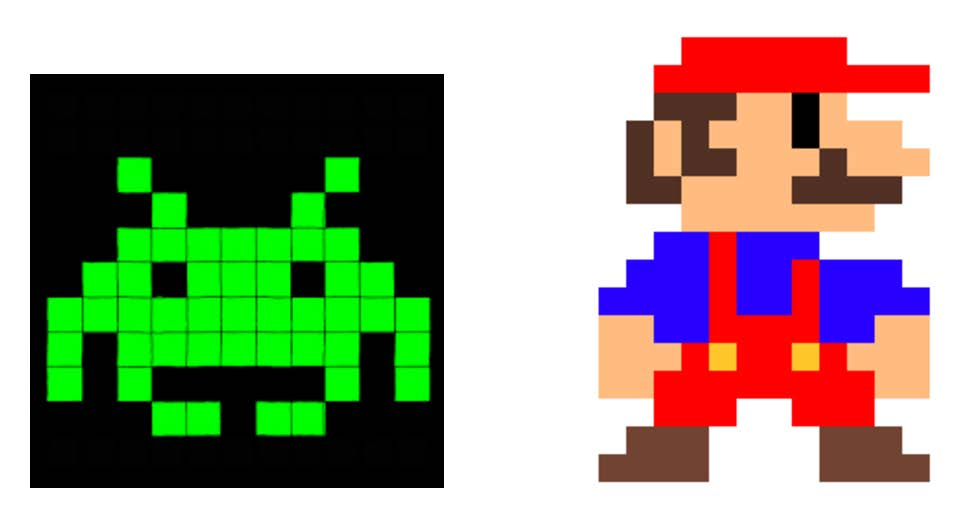
\includegraphics[width=0.5\columnwidth]{zooids-10.jpg}
    \caption*{图~10\hskip1em 1978年《太空侵略者》游戏中的外星人,1983年任天堂的《马里奥兄弟》游戏中的主要角色。}
\end{figure}

事物连续体也适用于传统的图形显示。 80年代的许多计算机显示器的分辨率都非常低(Sinclair ZX-81和Tandy TRS-80的半图形为64 48像素),因此像素是可辨认的粒子,就像我们之前的示例中的人畜共患动物一样(请参见图10)。现在,使用超高分辨率显示器,像素几乎变得不可见,即它们成为原子。但是,基于像素的显示和大量UI之间在概念上存在主要差异,我们将在下面讨论。

\subsection{显示形式: 固定 vs. 可移动元素}

\begin{figure}[htbp]
    \centering
    \includegraphics[width=0.5\columnwidth]{zooids-11.png}
    \caption*{图~11\hskip1em 通过使用(1)Bresenham算法和(2)自由对象定位来组合16个元素而获得的圆。}
\end{figure}

我们习惯于在计算机显示器上对图形进行编程,其中元素(像素)排列在规则的网格上,并且仅控制其颜色。尽管群体UI的元素也可以具有不同的颜色(在我们的系统中,每个动物群都嵌入了一个彩色LED),但是主要区别在于它们可以自由放置。即使两个系统之间的分辨率相同,元素组合成形状的方式也大不相同(见图11)。通常,与简单地打开和关闭像素相比,自由定位允许更好的形状控制。同时,这种额外的灵活性是以响应时间较慢和工程复杂性为代价的,并且存在诸如避免碰撞和优化元素-目标分配等算法问题。此外,对于只有很少动物等元素的系统,设计人员需要仔细考虑如何最佳地使用每个动物,就像80年代的设计人员必须仔细考虑如何最好地使用每个像素一样。随着大量UI分辨率的提高,它的关注将越来越少,但另一方面,工程和算法挑战可能会变得更加困难。此外,如图8所示,显示元素可以是同质的,如带动物的,也可以是异质的。

\subsection{显示形式: 固定数量元素 vs. 可变数量元素}

在常规的图形显示器上,像素的总数通常是固定的,并且通过简单地操纵像素颜色(例如,在白色背景上具有或多或少的深色像素)来实现在屏幕上具有更多或更少内容的错觉。相反,许多群体应用程序(例如,我们的绘图应用程序)要求元素的数量随时间实际变化。不能创建或销毁动物小动物,但是正如我们所看到的,未分配的动物小动物可以放置在专用区域中,并在需要时移动到工作区。这种类型的对象持久性有助于实现真实感,并可以帮助用户在视图更改中保持方向[7]。结果,对象持久性通常被实现为现代GUI中的隐喻(例如[44])。 Swarm UI本身就支持这些隐喻,它们迫使设计者考虑如何对外观和消失进行动画处理[7]。但是,当需要真实的外观和消失时,大量的UI可能是不切实际的,并且不断到达和离开的元素所产生的运动可能会分散最终用户的注意力。

\subsection{显示形式: 具有标识的元素 vs. 可互换的元素}

要进行的一个重要区别是,具有固定标识的大量UI元素与不可互换的元素之间。通常,用作“事物”的元素具有固定的标识,而构成“事物”的元素是可互换的。例如,在我们的形状绘制应用程序中,组成一个圆或一条线的动物标本没有自己的身份,可以自由交换。如实施部分所述,这可以优化群体界面,从而即使在复杂的过渡过程中,动物的运动也保持最小。同时,不希望将小部件(例如,手柄中的一个)与另一只动物类交换,因为这可能使用户感到迷惑,特别是如果她要抓住它。类似地,在每个动物群具有稳定含义的系统中(例如,一个动物群代表一个数据点的可视化系统),交换动物群会产生令人困惑或误导的动画。因此,群体UI的设计者应仔细考虑哪些元素是可互换的,以及应该为哪些元素赋予固定的标识。最后,永远不要重新分配被操纵的元素,这在我们当前的Zooid实现中会自动确保。

\subsection{交互:元素操纵}

常规的图形显示不允许对像素进行物理操作。尽管直接触摸显示器给人一种直接操作的感觉,但主观体验和表现力水平却不足以实现真正的物理对象操作[75]。相比之下,Zooids可以被抓住并直接被操纵,从而可以充分利用人类的手[34]。例如,在我们的群绘制方案中,用户不仅可以使用诸如控制点之类的替代物来操纵曲线,还可以直接对曲线进行整形。我们的系统通过记录触碰动物的时间并根据其位置不断更新其目标来明确支持此类交互。通常,大量的UI设计人员不仅应该关注“综合”交互的设计,而且还应该考虑纯物理交互方面的可能性[28]。由于它们的形状因素,可将Zooids既作为对象(东西)的集合,又作为单个对象(东西)进行操纵。随着群体用户界面元素的变小,负担能力将发生巨大变化。例如,大米可以单独处理,但是大米最好作为“原料”来处理。尽管在像我们这样的具有足够大元素的系统中本机支持对象操纵,但未来的成群用户界面将需要能够将多个元素合并为实体对象,以支持类似操纵。

\subsection{互动:元素的不同作用}

可以为不同的swarm UI元素赋予不同的角色。例如,在我们的时间序列可视化应用程序中,顶部的动物群仅用于显示目的,而底部的动物群用作控制器。相比之下,在绘图应用程序中,尽管不同的动物对输入的解释也不同,但动物和动物都用于输入和输出。例如,在我们的矩形绘图工具中,移动两个控制点可以重塑矩形,而移动任何其他动物模型都可以对其进行转换。为不同的swarm UI元素赋予不同的角色可以提高设计的灵活性,但同时也带来了如何传达能力的问题。在我们的示例应用程序中,我们将不同的LED颜色分配给不同的功能,但是颜色映射是任意的,并且该方法假定已经熟悉系统的用户。通过给不同的人畜共患病动物提供不同的形状,可以更好地提供食物,这与TUI设计的传统一致[13]。这些不同的形状可能是可裁剪的,或者说,Zooids可以动态改变其形状。但是,对于高分辨率群体UI,更自然的方法是通过将许多粒子或原子组装在一起来生产不同形状的对象,如我们先前所讨论的。

\subsection{环境:额外的视觉反馈}

尽管我们说明的绘图应用程序是纯集群用户界面,但实际上,许多粗粒度的集群用户界面都需要显示额外的可视信息(例如文本)才能真正使用。我们举例说明了两种方法:一种可以制作包含所有必要注解的支撑表面,只要这些注解随着时间的推移是稳定的(例如在棋盘游戏中)。当注释需要随时间变化时,可以将动物标本放置在常规的图形显示器上,或者,如果光学跟踪在红外光谱中,则可以使用顶部投影。尽管当前需要额外的显示硬件,但与传统的TUI相比,Zooids可以自己传达更多的视觉信息,而传统的TUI仅仅包含一些有形的控制器,并且通常会通过其他图形叠加来传达大多数视觉信息。可以想象,未来的大量用户界面将具有足够的高分辨率,能够充当其自己的显示,从而完全消除了对虚拟信息叠加的需求,而虚拟叠加信息会遇到许多问题,例如(用于顶部投影)遮挡,校准困难,并且难以在发亮或黑暗的表面上投射[17]。

\section{局限性和未来工作}

Zooids系统存在许多技术限制,限制了其作为群用户界面的功能和性能。这些范围从设备的规模和速度到成本。

一个重大限制是我们的机器人具有非完整的驱动器,这意味着它们无法在二维空间中自由移动,而必须转向特定方向,例如汽车。具有全向驱动的完整系统将使机器人能够更平稳地移动,并且更容易响应用户交互。与使用机器人作为显示器的情况不同,可以预先计算运动路径[63],我们的交互系统可能无法找到简单或可理解的路径,尤其是当运动距离较小时。

当前,我们的输入感测仅限于每个机器人周围的电容式触摸输入。一次与许多动物接触时,并不是所有的触摸传感器都会被激活,只有那些直接触摸用户手的触摸传感器才会被激活。传感器融合技术可用于识别和匹配两个或多个正在一致移动的机器人之间的运动。这将允许同时利用许多机器人的直接操纵的更丰富的交互技术。

我们系统的另一个技术限制是它使用外部投影仪进行跟踪。该要求增加了成本,并且还需要额外的硬件和设置才能使用该系统,从而阻碍了动物类的可扩展性。此外,像所有光学跟踪系统一样,我们的系统也受到与系统交互时经常发生的种种限制。最后,我们的投影仪和光电二极管在光谱范围内工作,因此很难在过多的环境光下使用(可以通过使用IR投影仪和光电二极管来改善这一点)。许多不同的方法可以改善我们的跟踪。与Valve的Vive Lighthouse跟踪器(http://www.htcvive.com)相似,使用旋转IR激光线信标可以大大降低成本,而拥有多个信标则可以解决某些遮挡问题。但是,我们看到了无线跟踪的巨大潜力,它可以减少设置,而只需添加少量固定信标(锚),即可根据接收到的无线电信号强度进行定位。或者,未来通过轮编码器和IMU之间的传感器融合改进航位推测定位技术的工作,再加上IR或RSSI元素之间无锚定点的定位,可以完全减少对外部跟踪的需求。我们认为,技术的进步将使大量的UI受益,从而允许更多的无所不在的安装。

许多机器人的电源和充电管理面临许多挑战。当前,我们的系统依赖于每个机器人必须手动放置的单独充电器。一个自动系统(可能在每个机器人中集成了无线充电线圈)可以让机器人在需要时通过返回充电基站自动进行充电。

当前系统中元素的规模和数量限制了交互类型和可以创建的应用程序-越来越少的元素可能允许与“事物”(而非“事物”)进行根本不同和更丰富的交互样式。为了实现更小的元件,我们将需要从带齿轮的直流齿轮电动机上移开,以便运动到其他致动装置,例如压电致动器。已经开发出了其他微型机器人,它们利用压电致动的顺应性联动装置,以较小的比例产生类似于小昆虫的运动[65],然而,这种规模的电力电子技术仍然具有挑战性[69]。限制机器人数量的另一个因素是成本。我们目前的小批量生产机器人设计,每个机器人的零件和组装成本约为50美元。在研究应用之外,这使得超过30至40的成本高昂。随着大规模生产的进一步设计,可以降低每台机器人的价格,但是其他制造技术,例如可打印和可折叠的机器人[11],最终可能会实现便宜得多的群体接口系统。

另一个很大的限制是交互区域以及元素可以在其上移动的表面的类型。由于类人动物的运动依赖于一组小的橡胶轮,因此我们的系统只能以最小的牵引力在相对平坦的表面上工作。这将我们的系统限制为2D交互。显然,对空中无人机群的研究[33]提供了制作完整3D接口的机会。但是,我们看到了进一步探索基于地面的群体接口的巨大机会,这些接口可能能够重新配置为2.5D甚至3D显示器。从蚂蚁和其他昆虫那里汲取灵感,它们可以通过交织和连接,甚至在彼此之上滚动而形成复杂的形状[8,59]。我们还看到了不同类别的机器人的巨大潜力,这些机器人可以帮助构造更多的3D形状,例如坡道机器人或其他可以使群体接口形成更复杂结构的无源构建块,类似于群体机器人的最新工作[79]。

最后,我们想探索更多的应用领域。现在我们已经创建了一个可扩展的平台,我们可以探索并快速制作原型。我们认为信息可视化是一个令人兴奋的领域,特别是对于创建参与度和教育领域而言。与传统的GUI相比,更好地了解大量用户界面的优缺点也很重要。为此,进行用户研究将确定使用群体用户界面的有利条件。我们希望我们的开源平台还能够鼓励其他研究人员,设计师和教育工作者探索各种应用,并将能够进一步评估和研究切实的交互作用原理。

\section{结论}

我们引入了群体用户界面,这是一类新的用户界面,由“集体移动并对用户输入做出反应的独立自走元素”组成。 我们描述了Zooids的技术实现,Zooids是一种用于构建群体用户界面的新型开源平台,并通过具体示例说明了其可能性。 我们希望本文和Zooids平台能够刺激更多的用户界面研究,并使我们更接近Sutherland和Ishii对最终用户界面的愿景,该愿景能够将人类的物理操作能力与计算能力完全结合在一起。

有关实施Zooid的所有必要材料和文档,请参见

https://github.com/PhysicalInteractionLab/SwarmUI/。

\section{参考文献}

